% =============================================================================
% SECTION 4 -- THE AI LANDSCAPE
% =============================================================================

\section{The AI Landscape}
\subsection{The Umbrella Term}

% ---------------------------------------------------------------------------
% 4.1  AI is an umbrella term
% ---------------------------------------------------------------------------
\begin{frame}{AI is an umbrella term}{what I work in: LLMs}
    \begin{columns}
        \begin{column}{0.5\textwidth}
            \begin{center}
                \begin{tikzpicture}
                    % canopy
                    \draw[accentcyan,very thick] (-2.6,0) arc (180:0:2.6);
                    % ribs
                    \draw[softgray,thick] (-2.2,1.39) -- (0,0);
                    \draw[softgray,thick] (-1.1,2.36) -- (0,0);
                    \draw[softgray,thick] (1.1,2.36) -- (0,0);
                    \draw[softgray,thick] (2.2,1.39) -- (0,0);
                    % handle
                    \draw[fgwhite,very thick] (0,0) -- (0,-1.9);
                    \draw[fgwhite,very thick] (0,-1.9) .. controls (0.75,-1.9) and (0.95,-1.45) .. (0.95,-1.2);
                    % AI label
                    \node[text=neonyellow,font=\semiLarge\bfseries] at (0,1.55) {AI};
                    % strings + sub-fields
                    \draw[neongreen,thick] (-2.2,1.39) -- (-2.2,-0.25);
                    \draw[neongreen,thick] (-1.1,2.36) -- (-1.1,-0.25);
                    \draw[neongreen,thick] (2.2,1.39) -- (2.2,-0.25);
                    \node[text=neongreen,font=\scriptsize,align=center] at (-2.2,-0.55) {Machine\\[-0.1em] Learning};
                    \node[text=neongreen,font=\scriptsize,align=center] at (-1.1,-0.55) {Deep\\[-0.1em] Learning};
                    \node[text=neongreen,font=\scriptsize,align=center] at (2.2,-0.55) {LLMs\\[-0.1em] (GenAI)};
                \end{tikzpicture}
            \end{center}
            \begin{itemize}[<+->]
                \item \glow{AI} = the umbrella over everything "intelligent".
                \item What I work in: \glow[neongreen]{LLMs} --- \emph{next-token predictors}.
            \end{itemize}
        \end{column}
        \begin{column}{0.45\textwidth}
            \begin{center}
                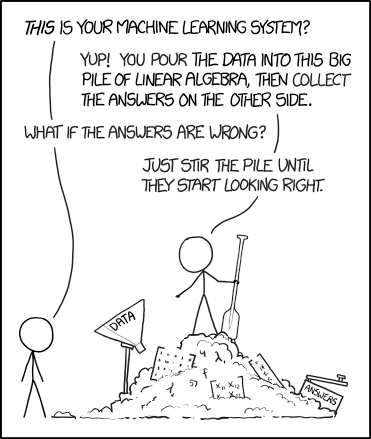
\includegraphics[height=3.9cm]{assets/img/xkcd_machine_learning.png}\\[0.15em]
                {\tiny\color{softgray}xkcd 1838 --- machine learning, the honest version}
            \end{center}
        \end{column}
    \end{columns}
\end{frame}

% ---------------------------------------------------------------------------
% 4.2  LLMs = next-token predictors
% ---------------------------------------------------------------------------
\subsection{Next-Token Predictors}

\begin{frame}{LLMs = next-token predictors}{everything ChatGPT does, one loop}
    \begin{columns}
        \begin{column}{0.56\textwidth}
            \begin{center}
                \begin{tikzpicture}[scale=0.78,transform shape]
                    % input tokens
                    \foreach \t/\x in {{The}/0,{cat}/1.2,{sat}/2.4,{on}/3.6,{the}/4.8} {
                        \node[draw=softgray,rounded corners=2pt,fill=darkgray,
                              minimum height=0.75cm,minimum width=1.0cm,
                              text=fgwhite,font=\small] at (\x,0) {\t};
                    }
                    % the unknown next token
                    \node[draw=accentcyan,rounded corners=2pt,fill=accentcyan!12,
                          minimum height=0.75cm,minimum width=1.0cm,
                          text=accentcyan,font=\small\bfseries] at (6.0,0) {?};
                    \draw[-{Stealth},thick,neonyellow] (6.7,0.55) -- (7.3,0.55);
                    % distribution over the next token
                    \node[text=fgwhite,font=\footnotesize] at (8.15,1.85) {$p$(next token)};
                    \foreach \t/\h/\y in {{mat}/1.55/0,{roof}/0.85/-0.65,{moon}/0.5/-1.3,{meow}/0.28/-1.95} {
                        \draw[fill=accentcyan,draw=accentcyan]
                            (7.55,\y) rectangle (7.55+\h*0.5,\y+0.42);
                        \node[text=fgwhite,font=\tiny] at (7.55+\h*0.5+0.32,\y+0.21) {\t};
                    }
                \end{tikzpicture}
            \end{center}
            \vspace{0.2cm}
            {\small \glow{Input:} a token sequence $\longrightarrow$ \glow[neongreen]{Output:} probabilities over the next token.}
        \end{column}
        \begin{column}{0.4\textwidth}
            \begin{itemize}[<+->]
                \item The model never \emph{searches} --- it \emph{predicts}.
                \item It repeats this loop, token by token, until you stop it.
                \item Add tools, and prediction becomes \glow[neongreen]{action}.
            \end{itemize}
            \onslide<4->{\begin{center}
                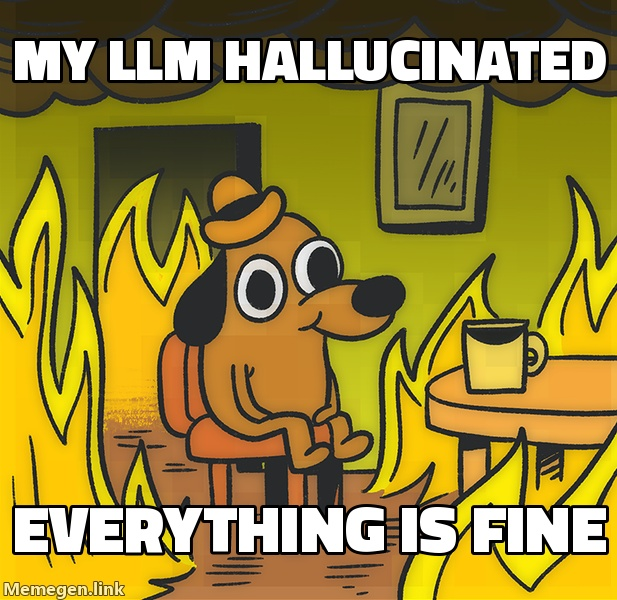
\includegraphics[height=3.1cm]{assets/img/meme_thisisfine.jpg}\\[0.1em]
                {\tiny\color{softgray}trust me bro --- I know this token}
            \end{center}}
        \end{column}
    \end{columns}
\end{frame}

% ---------------------------------------------------------------------------
% 4.3  the lens + the assistant axis
% ---------------------------------------------------------------------------
\subsection{The Lens \& The Assistant Axis}

\begin{frame}{Through the lens}{once you see it, you can't unsee it}
    \begin{columns}
        \begin{column}{0.55\textwidth}
            \begin{center}
                \begin{tikzpicture}
                    % background noise: all the buzzwords
                    \node[text=softgray,font=\footnotesize] at (0,1.05) {deep learning ~~ AGI ~~ neural nets ~~ reasoning};
                    \node[text=softgray,font=\footnotesize] at (0,0.35) {chatbots ~~ agents ~~ alignment ~~ RAG ~~ hype};
                    % magnifying glass
                    \draw[accentcyan,very thick] (1.15,0.25) circle (1.6);
                    \draw[accentcyan,very thick] (2.45,-1.05) -- (3.45,-1.95);
                    % lens content
                    \clip (1.15,0.25) circle (1.6);
                    \fill[bgdark] (1.15,0.25) circle (1.6);
                    \node[text=neonyellow,font=\semiLarge\bfseries] at (1.15,0.55) {next token};
                    \node[text=neonyellow,font=\semiLarge\bfseries] at (1.15,-0.1) {prediction};
                    \node[text=accentcyan,font=\footnotesize] at (1.15,-0.85) {$p(w_t \mid w_{<t})$};
                \end{tikzpicture}
            \end{center}
        \end{column}
        \begin{column}{0.4\textwidth}
            \begin{itemize}[<+->]
                \item The \glow[neonyellow]{lens}: look at any AI through it.
                \item \glow{Agents}? next-token prediction + tools.
                \item \glow{Alignment}? steering the same predictor.
                \item The hype is loud; the mechanism is simple.
            \end{itemize}
        \end{column}
    \end{columns}
\end{frame}

\begin{frame}{The assistant axis}{from chatbot to agent}
    \begin{center}
        \begin{tikzpicture}
            \draw[fgwhite,very thick,-{Stealth}] (0,0) -- (11.8,0);
            \foreach \x in {0.7,6.0,11.2} {
                \draw[accentcyan,thick] (\x,-0.15) -- (\x,0.15);
            }
            \node[text=fgwhite,font=\small] at (0.7,0.7) {Chatbot};
            \node[text=fgwhite,font=\small] at (6.0,0.7) {Assistant};
            \node[text=fgwhite,font=\small] at (11.2,0.7) {Agent};
            \node[text=softgray,font=\footnotesize] at (0.7,-0.65) {answers};
            \node[text=softgray,font=\footnotesize] at (6.0,-0.65) {does tasks for you};
            \node[text=softgray,font=\footnotesize] at (11.2,-0.65) {acts in your environment};
            \node[text=softgray,font=\footnotesize] at (0.7,-1.1) {0 tools};
            \node[text=softgray,font=\footnotesize] at (6.0,-1.1) {a few tools};
            \node[text=softgray,font=\footnotesize] at (11.2,-1.1) {many tools + memory};
            \draw[neonyellow,thick,dashed] (3.4,-0.45) -- (3.4,0.45);
            \node[text=neonyellow,font=\footnotesize] at (3.4,-1.75) {you are here today};
        \end{tikzpicture}
    \end{center}
    \pause
    \begin{center}
        {\small \glow{Question:} where do you want to live on this axis by the end of the year?}
    \end{center}
\end{frame}

% ---------------------------------------------------------------------------
% 4.4  the alignment wall
% ---------------------------------------------------------------------------
\subsection{The Alignment Wall}

\begin{frame}{The alignment wall}{a tiny corner of a huge research effort}
    {\small\color{fgwhite}Real research is happening on \glow{AI alignment} --- nine papers I keep going back to:}
    \vspace{0.25cm}
    \begin{center}
        \begin{tikzpicture}[
            papercard/.style={draw=softgray,rounded corners=3pt,fill=darkgray,
                              text width=3.35cm,align=left,inner sep=5pt,font=\tiny}]
            \node[papercard] (c11) at (0,0) {\textbf{Concrete Problems in AI Safety}\\[0.15em]
                \textcolor{softgray}{Amodei, Olah, et al.}\\[0.15em]
                \textcolor{accentcyan}{2016 $\cdot$ arXiv:1606.06565}};
            \node[papercard] (c12) at (3.95,0) {\textbf{AI Safety via Debate}\\[0.15em]
                \textcolor{softgray}{Irving, Christiano, Amodei}\\[0.15em]
                \textcolor{accentcyan}{2018 $\cdot$ arXiv:1805.00899}};
            \node[papercard] (c13) at (7.9,0) {\textbf{Scalable Agent Alignment via Reward Modeling}\\[0.15em]
                \textcolor{softgray}{Leike, Krueger, et al.}\\[0.15em]
                \textcolor{accentcyan}{2018 $\cdot$ arXiv:1811.07871}};
            \node[papercard] (c21) at (0,-1.9) {\textbf{Fine-Tuning LMs from Human Preferences}\\[0.15em]
                \textcolor{softgray}{Ziegler, Stiennon, et al.}\\[0.15em]
                \textcolor{accentcyan}{2019 $\cdot$ arXiv:1909.08593}};
            \node[papercard] (c22) at (3.95,-1.9) {\textbf{Training a Helpful \& Harmless Assistant (RLHF)}\\[0.15em]
                \textcolor{softgray}{Bai, Jones, et al.}\\[0.15em]
                \textcolor{accentcyan}{2022 $\cdot$ arXiv:2204.05862}};
            \node[papercard] (c23) at (7.9,-1.9) {\textbf{Constitutional AI: Harmlessness from AI Feedback}\\[0.15em]
                \textcolor{softgray}{Bai, Kadavath, et al.}\\[0.15em]
                \textcolor{accentcyan}{2022 $\cdot$ arXiv:2212.08073}};
            \node[papercard] (c31) at (0,-3.8) {\textbf{Towards Understanding Sycophancy}\\[0.15em]
                \textcolor{softgray}{Sharma, Tong, et al.}\\[0.15em]
                \textcolor{accentcyan}{2023 $\cdot$ arXiv:2310.13548}};
            \node[papercard] (c32) at (3.95,-3.8) {\textbf{Weak-to-Strong Generalization}\\[0.15em]
                \textcolor{softgray}{Burns, Izmailov, et al.}\\[0.15em]
                \textcolor{accentcyan}{2023 $\cdot$ arXiv:2312.09390}};
            \node[papercard] (c33) at (7.9,-3.8) {\textbf{The AI Alignment Paradox}\\[0.15em]
                \textcolor{softgray}{West \& Aydin}\\[0.15em]
                \textcolor{accentcyan}{2024 $\cdot$ arXiv:2405.20806}};
        \end{tikzpicture}
    \end{center}
    \vspace{0.2cm}
    \begin{center}{\tiny\color{softgray}every paper is free on arXiv --- pick one, read it tonight}\end{center}
\end{frame}

% ---------------------------------------------------------------------------
% 4.5  the paper that started the fourth wave
% ---------------------------------------------------------------------------
\begin{frame}{The paper that started this fourth wave}{Attention Is All You Need}
    \begin{center}
        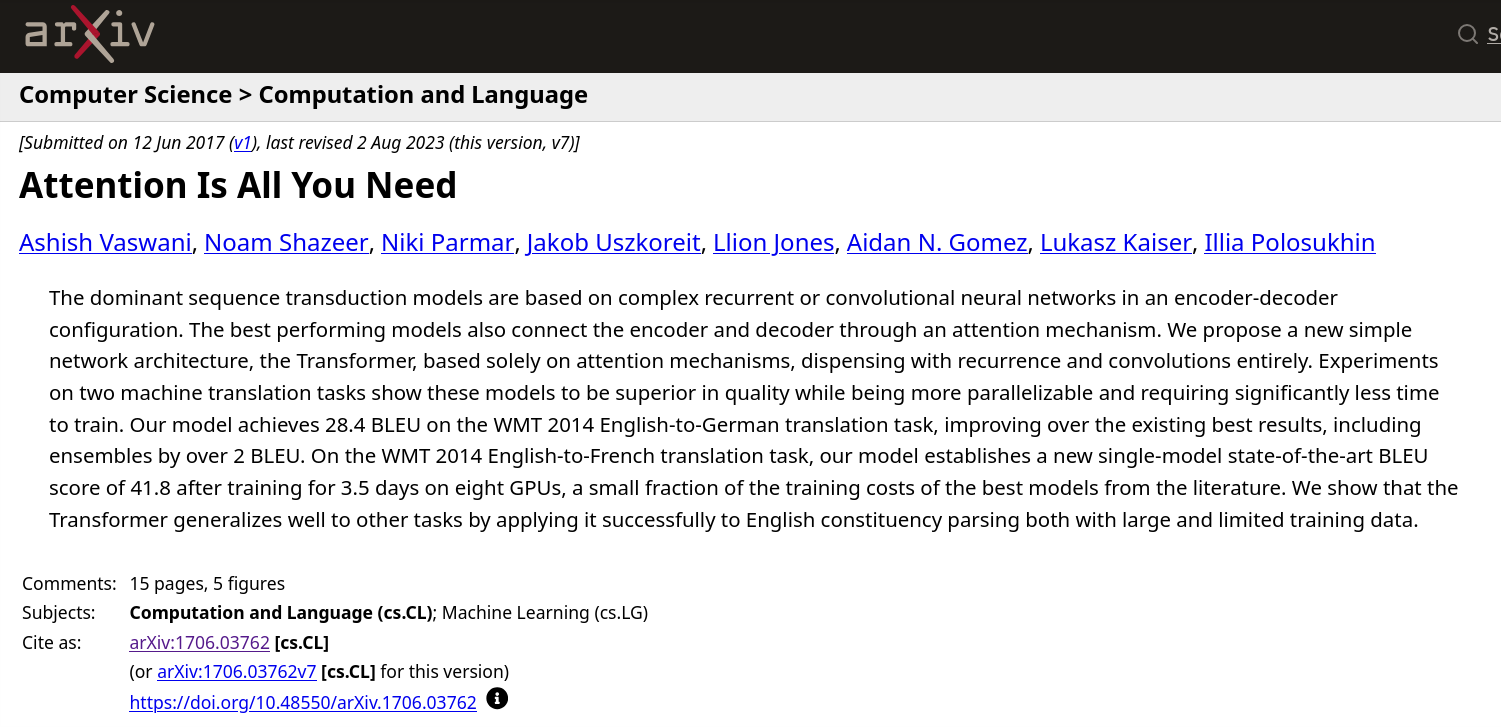
\includegraphics[height=5.2cm]{assets/img/attention_is_all_you_need.png}
        \vspace{0.25cm}

        {\small Vaswani et al., 2017 --- \glow{Attention Is All You Need}\\[0.1em]
         arXiv:1706.03762}
    \end{center}
\end{frame}
